\documentclass{article}
\usepackage{comment}
\usepackage[english]{babel}
\usepackage[utf8]{inputenc}
\usepackage{fancyhdr}
\usepackage[round]{natbib}
\usepackage{graphicx}
\usepackage{url}
\usepackage{amsmath}
\usepackage{amssymb}
\DeclareMathOperator*{\argmax}{argmax}
\pagenumbering{arabic}

\pagestyle{fancy}
\fancyhf{}
\rhead{Mohammad Rahmani}
\lhead{Text generation by artistic indexes}

\newcommand{\ignore}[1]{}
\begin{document}
	\bibliographystyle{plainnat}
	\title{Automatic, literary text generation by artistic indexes}
	\author{Mohammad Rahmani}
	\date{}
	\maketitle
	
	\section{Introduction} \label{sec:introduction}
	While numerous creative language generation studies, have focused on topics such as generating poems, stories, etc by learning from the corpora, few have addressed incorporation of artistic indexes (similar to indexes described in Section \ref{sec:related-works-artistic value-indexes}) in their generation process. The few which have done so, have counted on training the model to learn artistic value styles from the corpora which results in repetitive results similar to the structures in the corpora. As such, a model that can generate literary text by considering artistic indexes, is missing. This proposal first suggests application of semantic vector spaces to mathematically defining some artistic indexes and then application of stochastic gradient descent to generate language which incorporate maximum of the aforementioned artistic indexes. 
	
	\section{Objective} \label{sec:objective}
	%todo change this to how amny times and in what orders artistic indexes in section "relative works, artistic section must be so that a piece of text incorporates maximum artistic value?
	This proposal\footnote{A piece of code in Java (just for the sake of clean code Java is chosen to build the skeleton, otherwise Python or a mix of two could also be used) which is being updated continuously is available at this  git repository to help with better understanding the objective and the methodology: \\ \url{https://github.com/donkarlo/gissoo}. \\Additionally a UML class diagram is available at\\ \url{https://github.com/donkarlo/gissoo/blob/master/docs/assets/artisticness.png}} tries to address the absence of a creative, artistic text generation model by selecting dependency sequences derived from corpora such that the maximum artistic value is achieved through mathematically defining a set of artistic indexes using stochastic gradient descent.   
	That is, taking $D$ in the following equation as a set of extracted potential dependencies in form of subjects, verbs and objects from corpora
	\begin{equation}
	\begin{split}
	if \; E=\{e_1,...,e_q\} \;and\; V=\{v_1,...,v_p\} \; then
	\\
	D = \{d_f = (s_i,v_h,o_j)|s_i,o_j \in E , v_h \in V \}
	\end{split}
	\label{eq:space-of-possible-dependencies}
	\end{equation} 
	where $E$ is the set of extracted entities(subjects and objects) and V is the set of extracted verbs,
	then this proposal is trying to introduce dependency sequences such as: 
	\begin{equation}
	\begin{split}
	l_n = (d_t)_{t=1}^{n}
	\end{split}
	\label{eq:sequences-of-dependencies}
	\end{equation} 
	
	such that $a(l_n)$ in 
	\begin{equation}
		\begin{split}
			a(l_n) =  \sum_{k=1}^{m}a_k(l_n) 
		\end{split}
		\label{eq:comprehensive-artistic-function}
	\end{equation}
	maximizes where $a_k$ is a single artistic value index member in A as follows:
	\begin{equation}
	A=\{a_k:l_n\longrightarrow(0,1)|k\in\{1,...,m\}\}
	\label{eq:artistic-indexes}
	\end{equation}
	In Section \ref{sec:methodology-stochastic-gradient-descent}, a solution based on stochastic gradient will be suggested to study in this proposal to generate diverse sequences of dependencies such as the one presented in Equation \ref{eq:sequences-of-dependencies} with local maximum artistic value values in each run.
	\section {Related works} \label{sec:related-works}
	The following subsections are subjects which must be addressed in Section \ref{sec:methodology} as a part of the solution to accomplish the objectives of this proposal. This section is particularly important since not only it references previous works which might be used in Section \ref{sec:methodology}, but also, incorporates the definition of some terminologies applied in the rest of this proposal. 
	\subsection{Creative language generation}
	The closest literary form to the expected results of this research proposal are poems (Particularly haiku), although it does not put emphasis on any particular literary form. Most poem generation models learn and repeat artistic patterns from corpora such as \citet{daza-2016-automatic-text-generation-by-learning-from-literary-structures}. Some researchers tried to develop models to avoid such repetitions in favor of creativity \citep{wu-2019-evaluating-image-inspired-poetry-generation} Narratives in form of short stories are also close to such theme, specially the idea of extracting possible dependencies between objects in corpora to form stories from a subset of them, is presented in works such as \citet{mcintyre-2009-learning-to-tell-tales-a-data-driven-approach-to-story-generation} which introduces a rank-based solution to select dependency sequences with arbitrary lengths and psycho-linguistic indexes to evaluate the results. Moreover \citet{mcintyre-2010-plot-induction-and-evolutionary-search-for-story-generation} uses evolutionary algorithms instead of the rank-based approach introduced in \citet{mcintyre-2009-learning-to-tell-tales-a-data-driven-approach-to-story-generation}
	\subsubsection{Dependency extraction}
	\label{sec:related-works-dependency-extraction}
	Although Standford Dependencies \citep{schuster-2016-enhanced-english-universal-dependencies-an-improved-representation-for-natural-language-understanding-tasks} will be used to extract dependencies from corpora, yet other innovative solutions have been proposed. An approach to extract chains of dependencies as constituents of a story is proposed in  \citep{chambers-2008-unsupervised-learning-of-narrative-event-chains}.
	\citet{martin-2018-event-representations-for-automated-story-generation-with-deep-neural-nets} suggests an interesting neural approach for the same type of extraction for story generation.	
	\cite{de-marneffe-2014-universal-stanford-dependencies-a-cross-linguistic-typology} suggests an improved taxonomy to capture grammatical
	relations across languages, including morphologically rich ones.  \cite{nivre-2016-universal-dependencies-v1-a-multilingual-treebank-collection} has discussed solutions to extract dependencies further than subject-object relations. 
	\subsection{Artistic indexes} \label{sec:related-works-artistic value-indexes}
	In this section three artistic indexes are introduced which will be addressed in Sections \ref{sec:methodology-antonym-class-shifts}, \ref{sec:methodology-ambiguity-appeal} and \ref{sec:methodology-vad} as sub-sections of the suggested methodology. Certainly more indexes could be investigated, yet for the sake of feasibility of accomplishing the objectives of this proposal within the reasonable time for a PhD, just the following three artistic indexes will be studied.  
	\subsubsection{Transition between antonym semantic vector classes}
	Various transition between different or even antonym semantic classes is considered as a source of artistic value in several literary forms. Haiku is one such form (Figure \ref{fig:antonym-shifts-between-semantic-classes})\footnote{
		Inspired from  a haiku by Yosa Buson
		\\
		An old silent pond...
		\\
		A frog jumps into the pond,
		\\
		splash! Silence again.
	}. \citet{ono-2015-word-embedding-based-antonym-detection-using-thesauri-and-distributional-information} suggests a solution for antonym detection by word embedding. 
	\begin{figure}[h!]
		\centering
		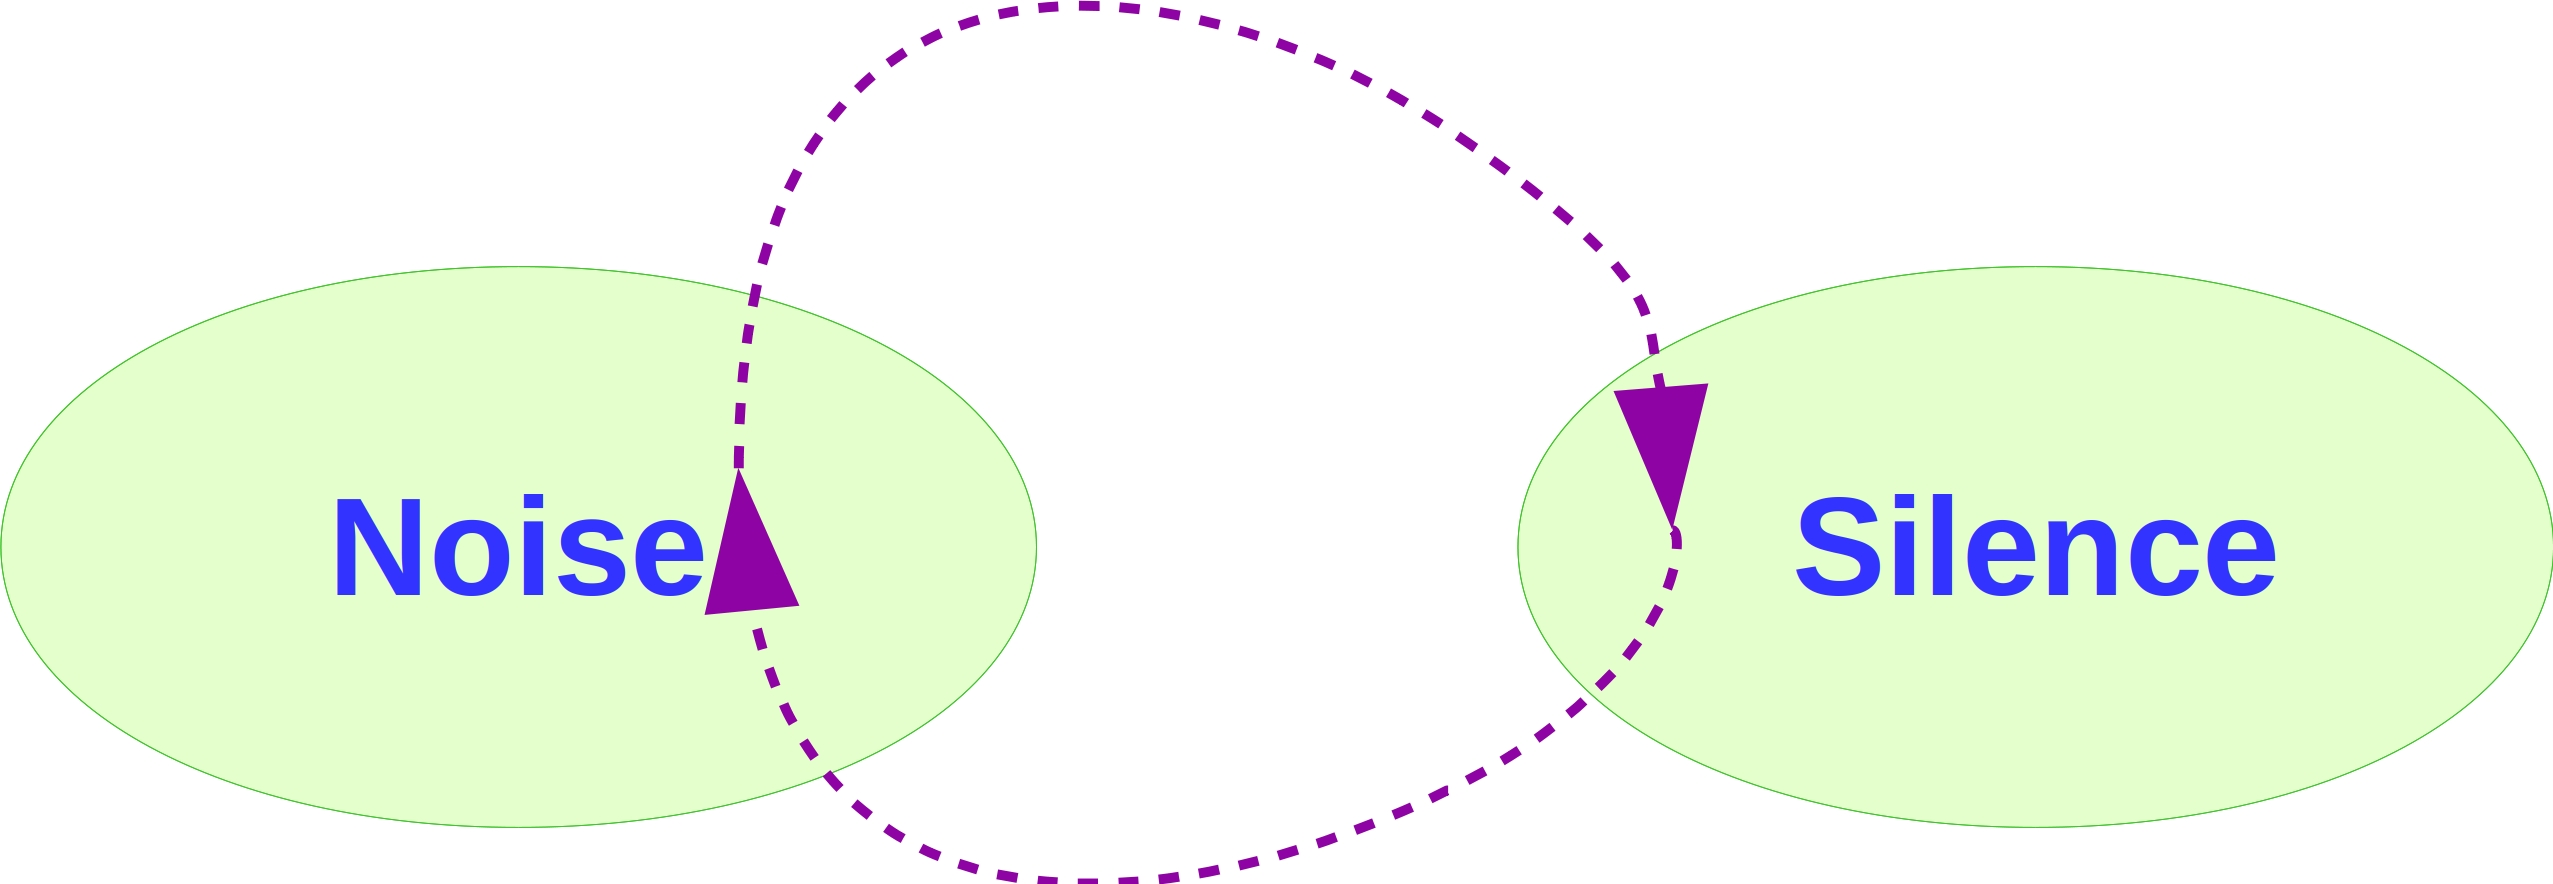
\includegraphics[width=0.6\textwidth]{/media/donkarlo/Elements/projs/research/assets/antonym-shifts-between-semantic-classes.jpg}
		\caption{Shift between antonym semantic classes. For example: [The] pond is silent. [A] Frog splash into it. [The] pond is silent [again]}
		\label{fig:antonym-shifts-between-semantic-classes}
	\end{figure}
	\subsubsection{Ambiguity}
	Ambiguity is an appealing constituent of an artifact \citep{muth-2015-the-appeal-of-challenge-in-the-perception-of-art-how-ambiguity-solvability-of-ambiguity-and-the-opportunity-for-insight-affect-appreciation}. For example, it is not determinable whether Mona Lisa is smiling and if she is, is it a bitter or a sweet smile? If the course of the events (dependencies) take the final perceived semantic to the border of two different semantic classes, then such ambiguity provokes imagination (Figure \ref{fig:ambiguity}). A subsequent result of ambiguity is suspense.
	\citet{cheong-2006-a-computational-model-of-narrative-generation-for-suspense} suggests a model to generate suspense. \citet{oneill-2011-toward-a-computational-framework-of-suspense-and-dramatic-arc} presents a suspense detection system based on the correlation between perceived likelihood of a protagonist’s failure and the amount of suspense reported by the audience.
	\begin{figure}[h!]
		\centering
		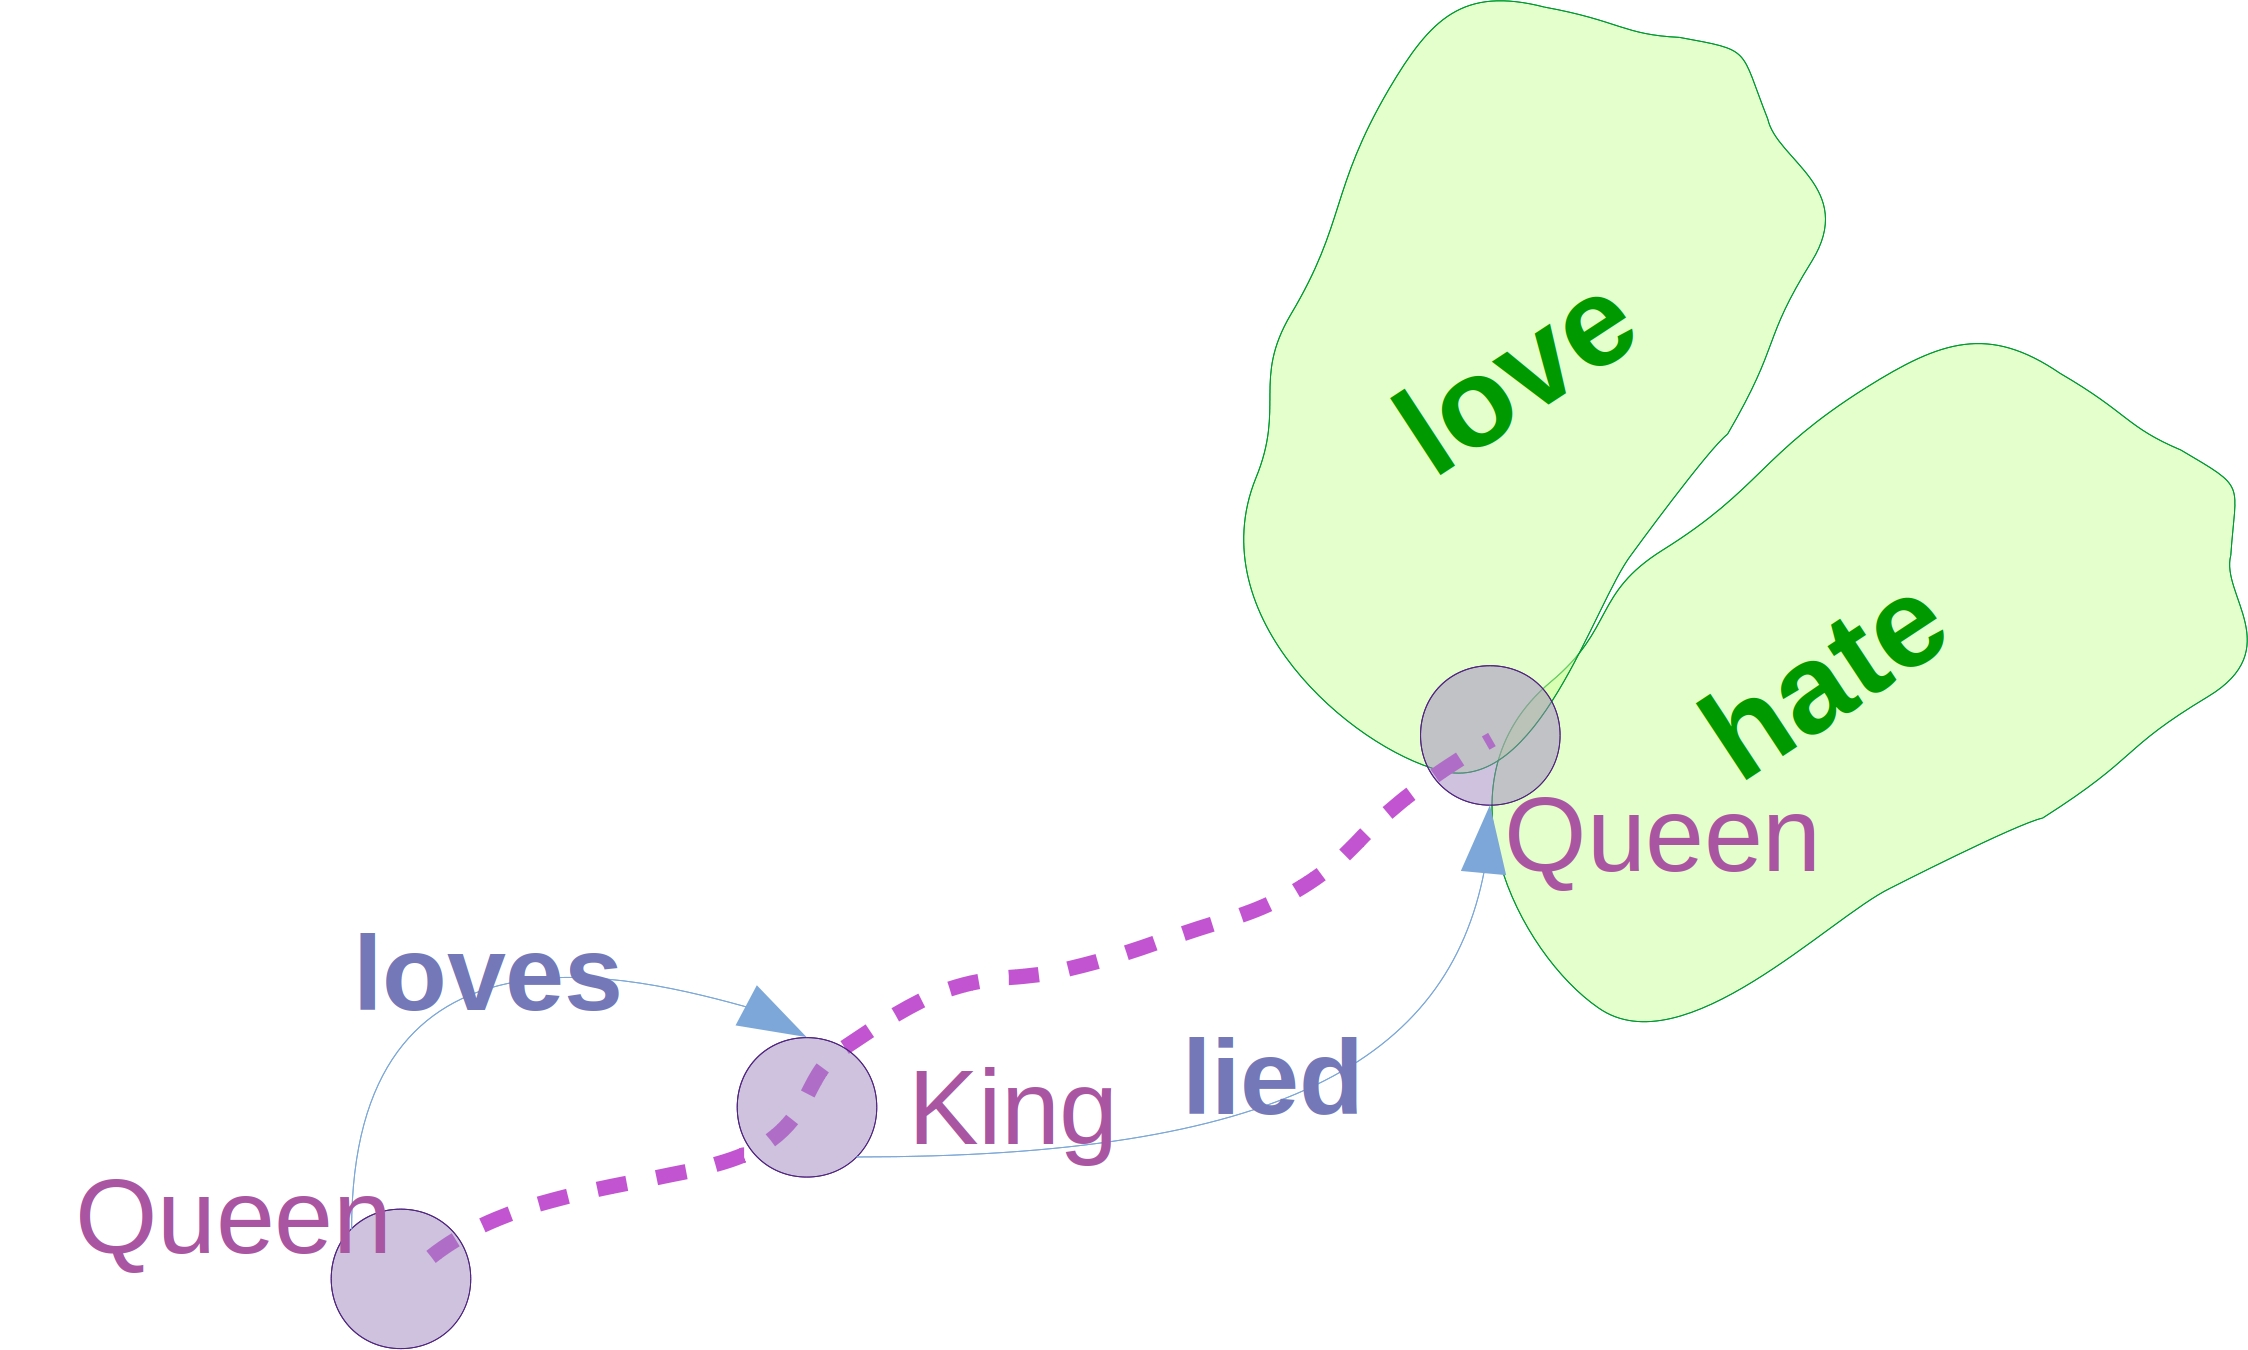
\includegraphics[width=0.6\textwidth]{/media/donkarlo/Elements/projs/research/assets/ambiguity.jpg}
		\caption{A dependency sequence which is ended in an ambiguity between "love" and "hate" in a story such as: "The queen loves the king, but the king lied the queen."} 
		\label{fig:ambiguity}
	\end{figure}
	\subsubsection{Valence, arousal and dominance (VAD) gravity of dependency sequences}
	Whenever the course of the events takes the situation to a semantic class from which escaping is impossible then the audience mind deeply engages with imagining potential break outs. For example, if the course of the events in the story, ends in a deep regret (\ref{fig:semantical-class-shift}), then however much a story character commits possible verbs, s/he can not change the semantic class from regret to something different (such as happiness ....). Naturally, such endings engages the imagination of the audience (reader) to think of ways with which the character can release himself from such situations. \citet{buechel-2016-feelings-from-the-past-adapting-affective-lexicons-for-historical-emotion-analysis} suggests a method to assign a VAD value to a sequence of sentences. Studies such as \citet{agrawal-2018-learning-emotion-enriched-word-representations,mao-2019-sentiment-aware-word-embedding-for-emotion-classification} and 
	\citet{li-2017-inferring-affective-meanings-of-words-from-word-embedding} have regarded VAD from a semantic vector perspective. \citet{li-2017-inferring-affective-meanings-of-words-from-word-embedding} suggests an embedding particular to affective meaning which includes the arousal and valence of the affection.
	\begin{figure}[h!]
		\centering
		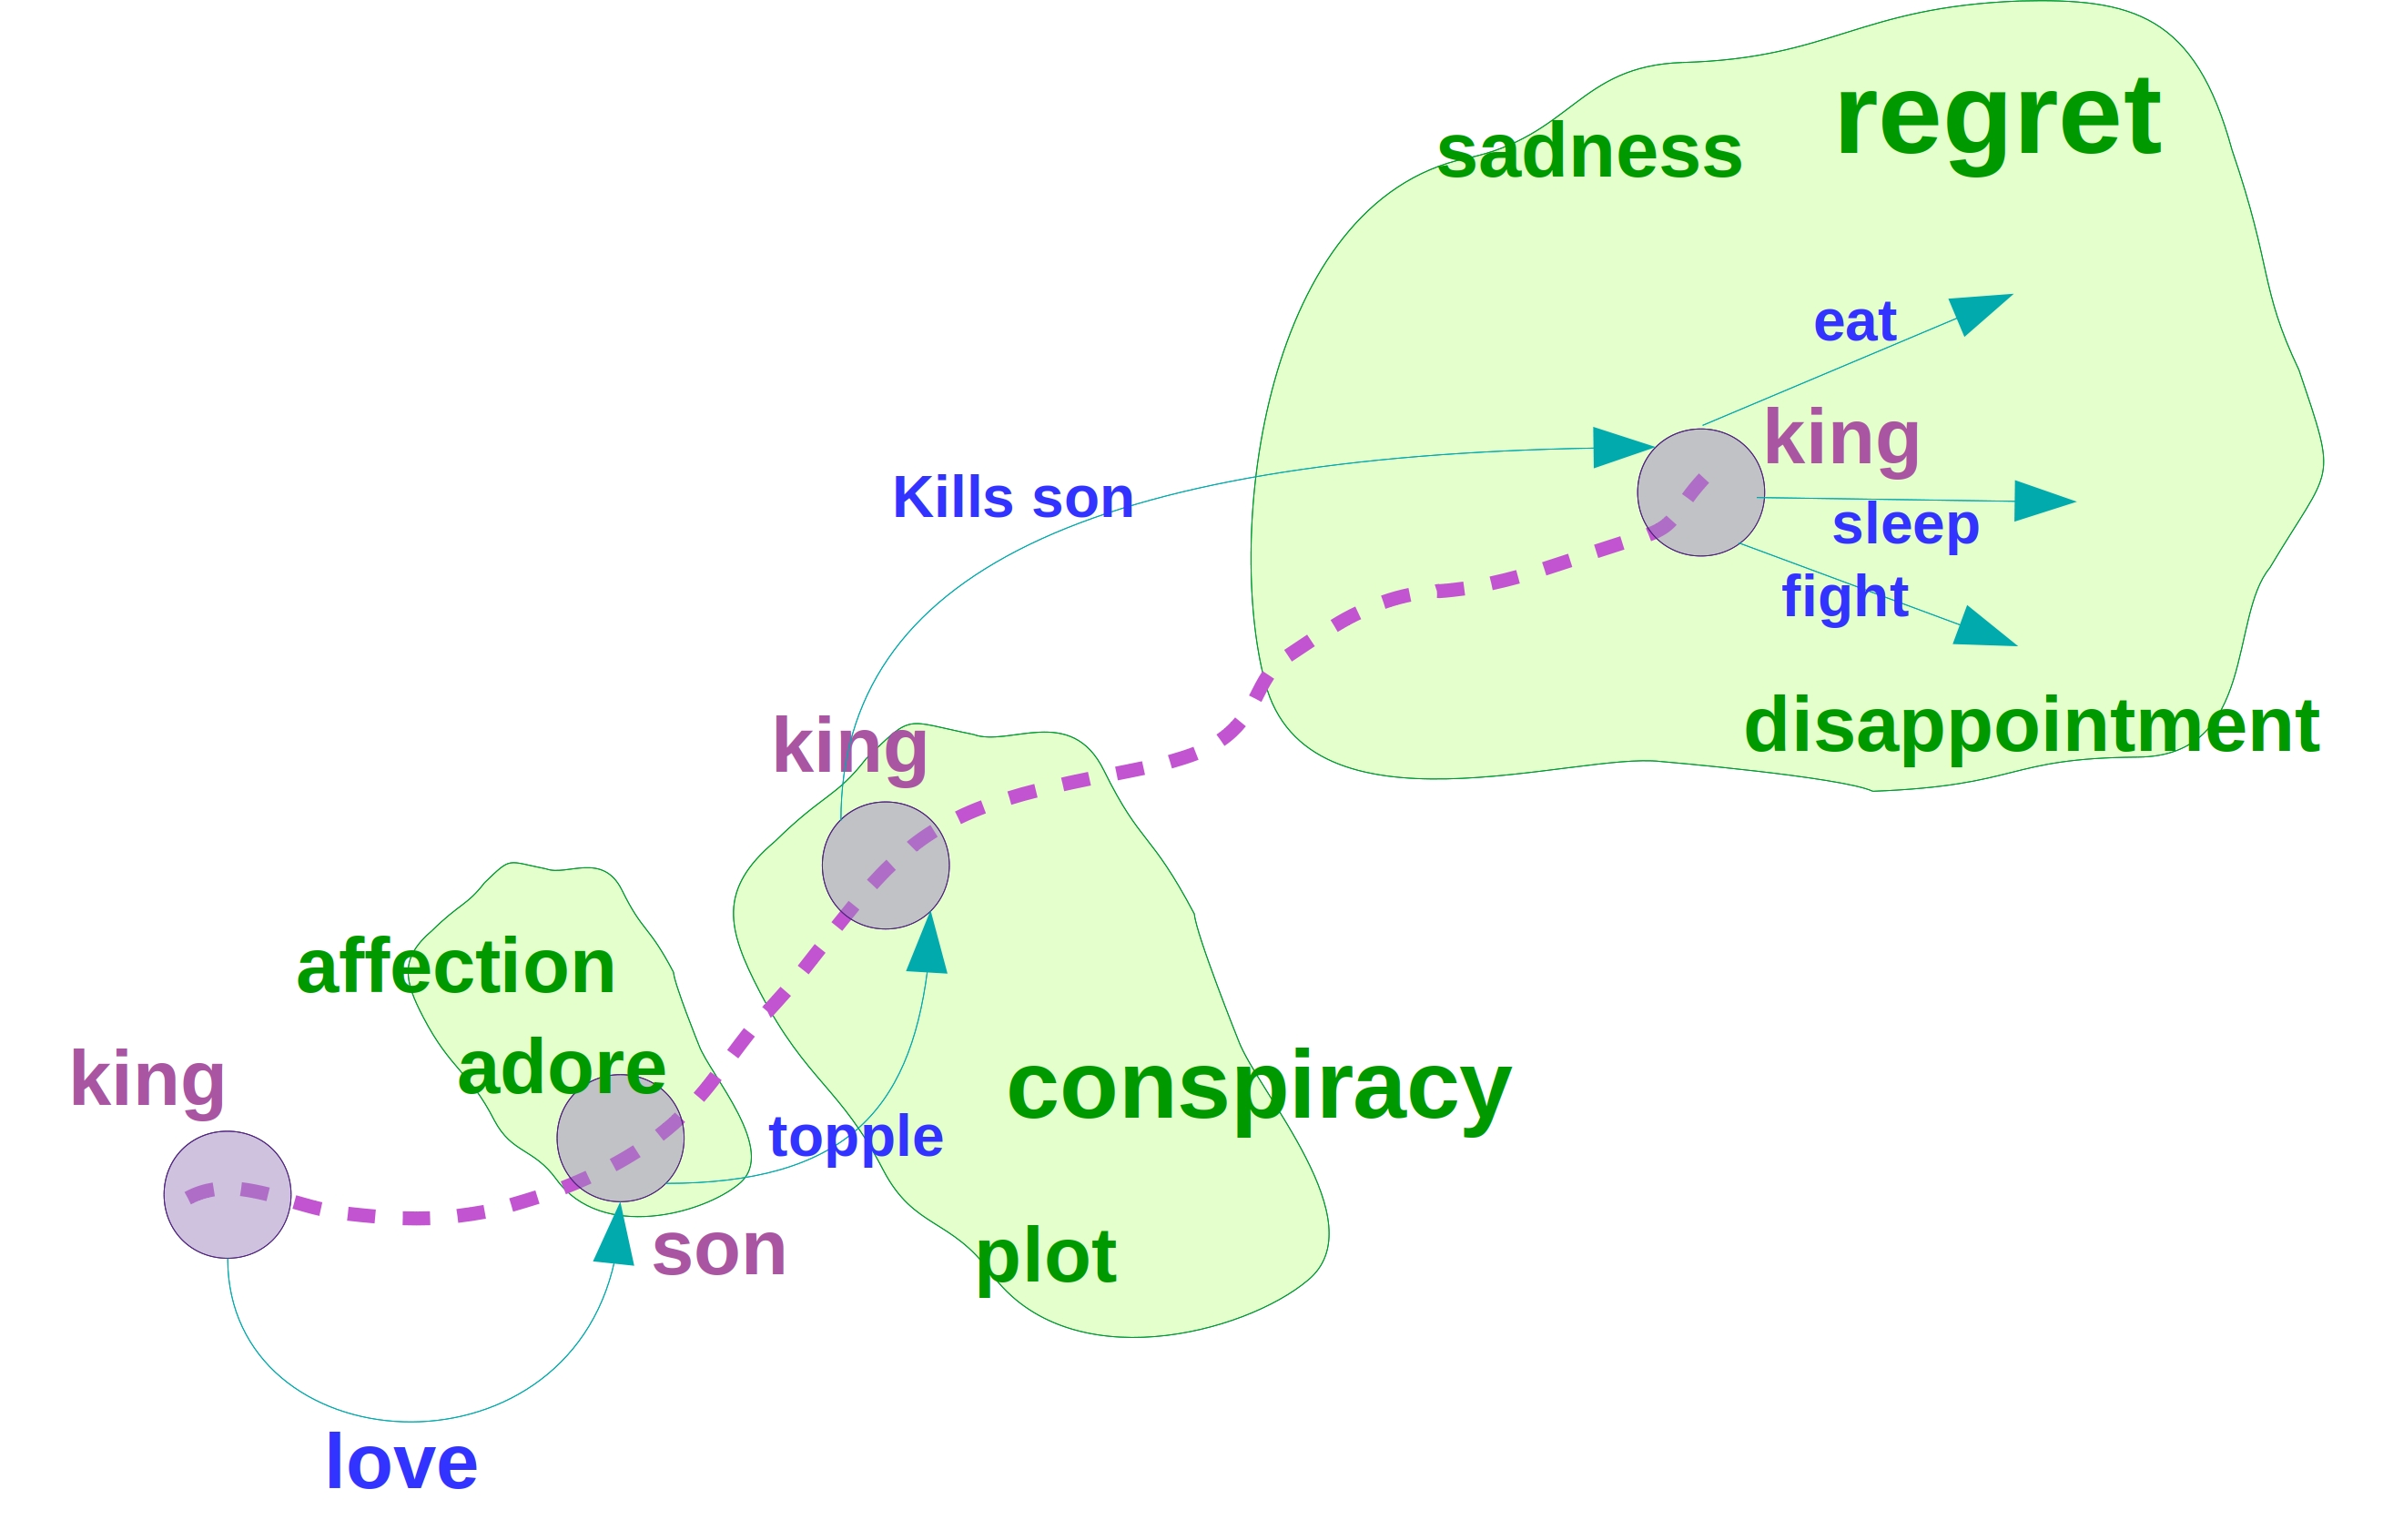
\includegraphics[width=1\textwidth]{/media/donkarlo/Elements/projs/research/assets/vad-semantics.jpg}
		\caption{Dependency sequence ultimately shifts to a semantic class(regret) in a story such as "The king loves his son. The son wants to topple the king. The king kills his son." with such a huge VAD that no other dependency in D can pull it out.} 
		\label{fig:semantical-class-shift}
	\end{figure}
	
	
	\subsection{Dependency (event) embedding} \label{sec:related-works-dependeny-embedding}
	There are some solutions which have been proposed toward event embedding such as
	\citet{weber-2018-event-representations-with-tensor-based-compositions}. Taking a dependency in $D$ as an event, such solutions are also applicable for dependencies. 
	
	\subsection{Application of stochastic gradient for text generation} 
	Previous to this proposal, it seems that no other study has used stochastic gradient descent to generate a dependency sequences with maximum artistic value values. Previously, studies such as  \citep{welleck-2019-neural-text-generation-with-unlikelihood-training,wellek-2019-non-monotonic-sequential-text-generation,welleck-2019-neural-text-generation-with-unlikelihood-training} have used neural approaches in generation of diverse texts with similar inputs, yet stochastic gradient descent, due to its nature seems to be also a feasible solution for such objectives.   
	
	\subsection{Surface realization} \label{sec:related-works-surface-realization} 
	Many surface realizers have been developed in recent years by taking advantage of neural methods. There are a wide range of modern, neural based Grammar, template  or statistical based methods are available but simple old solutions such as \cite{lavoie-1999-a-fast-and-portable-realizer-for-text-generation-systems} can be used for primary tasks in this proposal.  
	
	\section{Methodology} \label{sec:methodology}
	Briefly, the methodology is composed of choosing a textual corpora from which a corpus of dependencies could be extracted and then introducing dependency sequences from $D$ such that they locally maximize the artistic indexes introduced in Section \ref{sec:related-works-artistic value-indexes} by taking advantage of stochastic gradient descent. In details:
	\subsection{Corpora building}
	\paragraph{Choosing textual Corpora} A corpora such as Wikipedia which doesn't inherently incorporate literary text will be used for dependency extraction. The reason for such a choice is to remove the bias that the model is learning its artistic value values from the corpora. 
	\paragraph{Dependency parsing} Stanford coreNLP dependency parser will be used to extract dependencies from corpora. If necessary, other neural models (such as those introduced in Section \ref{sec:related-works-dependeny-embedding}) will also be used for more complex requirements. 
	\subsection{artistic indexes} \label{sec:methodology-artistic value-indexes}
	In this phase a set of artistic indexes will be mathematically defined so that sequences such as $l_n$ in Equation \ref{eq:sequences-of-dependencies} can be mapped to corresponding artistic value values between 0 and 1 as described in Equation \ref{sec:related-works-dependeny-embedding}.
	\subsubsection{Transition between antonym vector semantic classes}\label{sec:methodology-antonym-class-shifts}
	First, a semantic vector space will be developed such that antonym words or dependencies are placed in different classes ( As a starting point, previous studies such as \citet{ono-2015-word-embedding-based-antonym-detection-using-thesauri-and-distributional-information} will be considered). Then, a model must be developed or trained %todo what refs?% 
	to detect the shifts between antonym semantic classes in a sequence of dependencies.    
	
	\subsubsection{Ambiguity} \label{sec:methodology-ambiguity-appeal}
	First a clustering model should be developed to cluster the words such that on the one hand, verbs can shift perceived meanings by the reader from dependencies in a sequence to  a vector-defined position in a final residential class (such as Figure \ref{fig:ambiguity}) and on the other hand, words with similar meanings cluster into same classes. Another model should be developed to measure the distance between the landing site of a dependency sequence meaning in its residence class and its neighboring classes. A dependency sequence with average closer distance to more classes is considered more ambiguous and consequently more artistic.  
	
	\subsubsection{Valence, arousal and dominance (VAD) gravity of dependency sequences} \label{sec:methodology-vad}
	A semantic vector space should be developed such that the resulting classes can adjust their extension according to the course of dependency sequences so that the size of verb vectors comply in a way that irrelevant verbs to the situation lose size while others grow in size. 
	
	\subsection{Stochastic gradient descent for dependency sequence generation}\label{sec:methodology-stochastic-gradient-descent} A dependency(event) embedding such as 
	\begin{equation}
	\begin{split}
	b:d_t\longrightarrow \mathbb{R}^z
	\\
	d_t\longrightarrow\vec{d_t}
	\end{split}
	\label{eq:script-embedding-function}
	\end{equation} 
	will be developed and will be used (using one of the solutions mentioned in Section \ref{sec:related-works-dependeny-embedding}) to map dependencies in $D$ to vectors. Taking advantage of stochastic gradient descent and the three aforementioned artistic indexes, a random or arbitrary dependency vector such as $\vec{d_i} \in \vec{D}$ will be given to a stochastic gradient descent function for maximizing Equation \ref{eq:comprehensive-artistic-function}. The next dependency embedding will be chosen by stochastic gradient descent along the partial derivative direction until $a(l_n)$ reaches a local maximum. As such, a sequence of dependencies will be introduced with maximum artistic indexes (Figure \ref{fig:dependency-gradient-descent}). Since the first dependency is chosen arbitrarily or randomly, then every time the first dependency changes, a new trajectory(sequence) of dependencies toward the local artistic value maximum is introduced. Such trajectory can be even more diversified when Equation \ref{eq:comprehensive-artistic-function} has more than one local maximum. As stochastic gradient descent's steps number toward reaching a maximum values is not predictable, then another advantage of this approach is generation of dependencies with unknown lengths.
	It is noticeable that the three artistic indexes may contradict each other. In other words, in some cases they defuse each other. For example, ambiguity appeal may inherently defuse antonym shifts because one is based on ending a dependency sequence between two contradicting semantic classes while the other is the matter of landing dependency members in distinct antonym classes. As such, existence of local maximums seems to be inevitable.      
	\begin{figure}[h!]
		\centering
		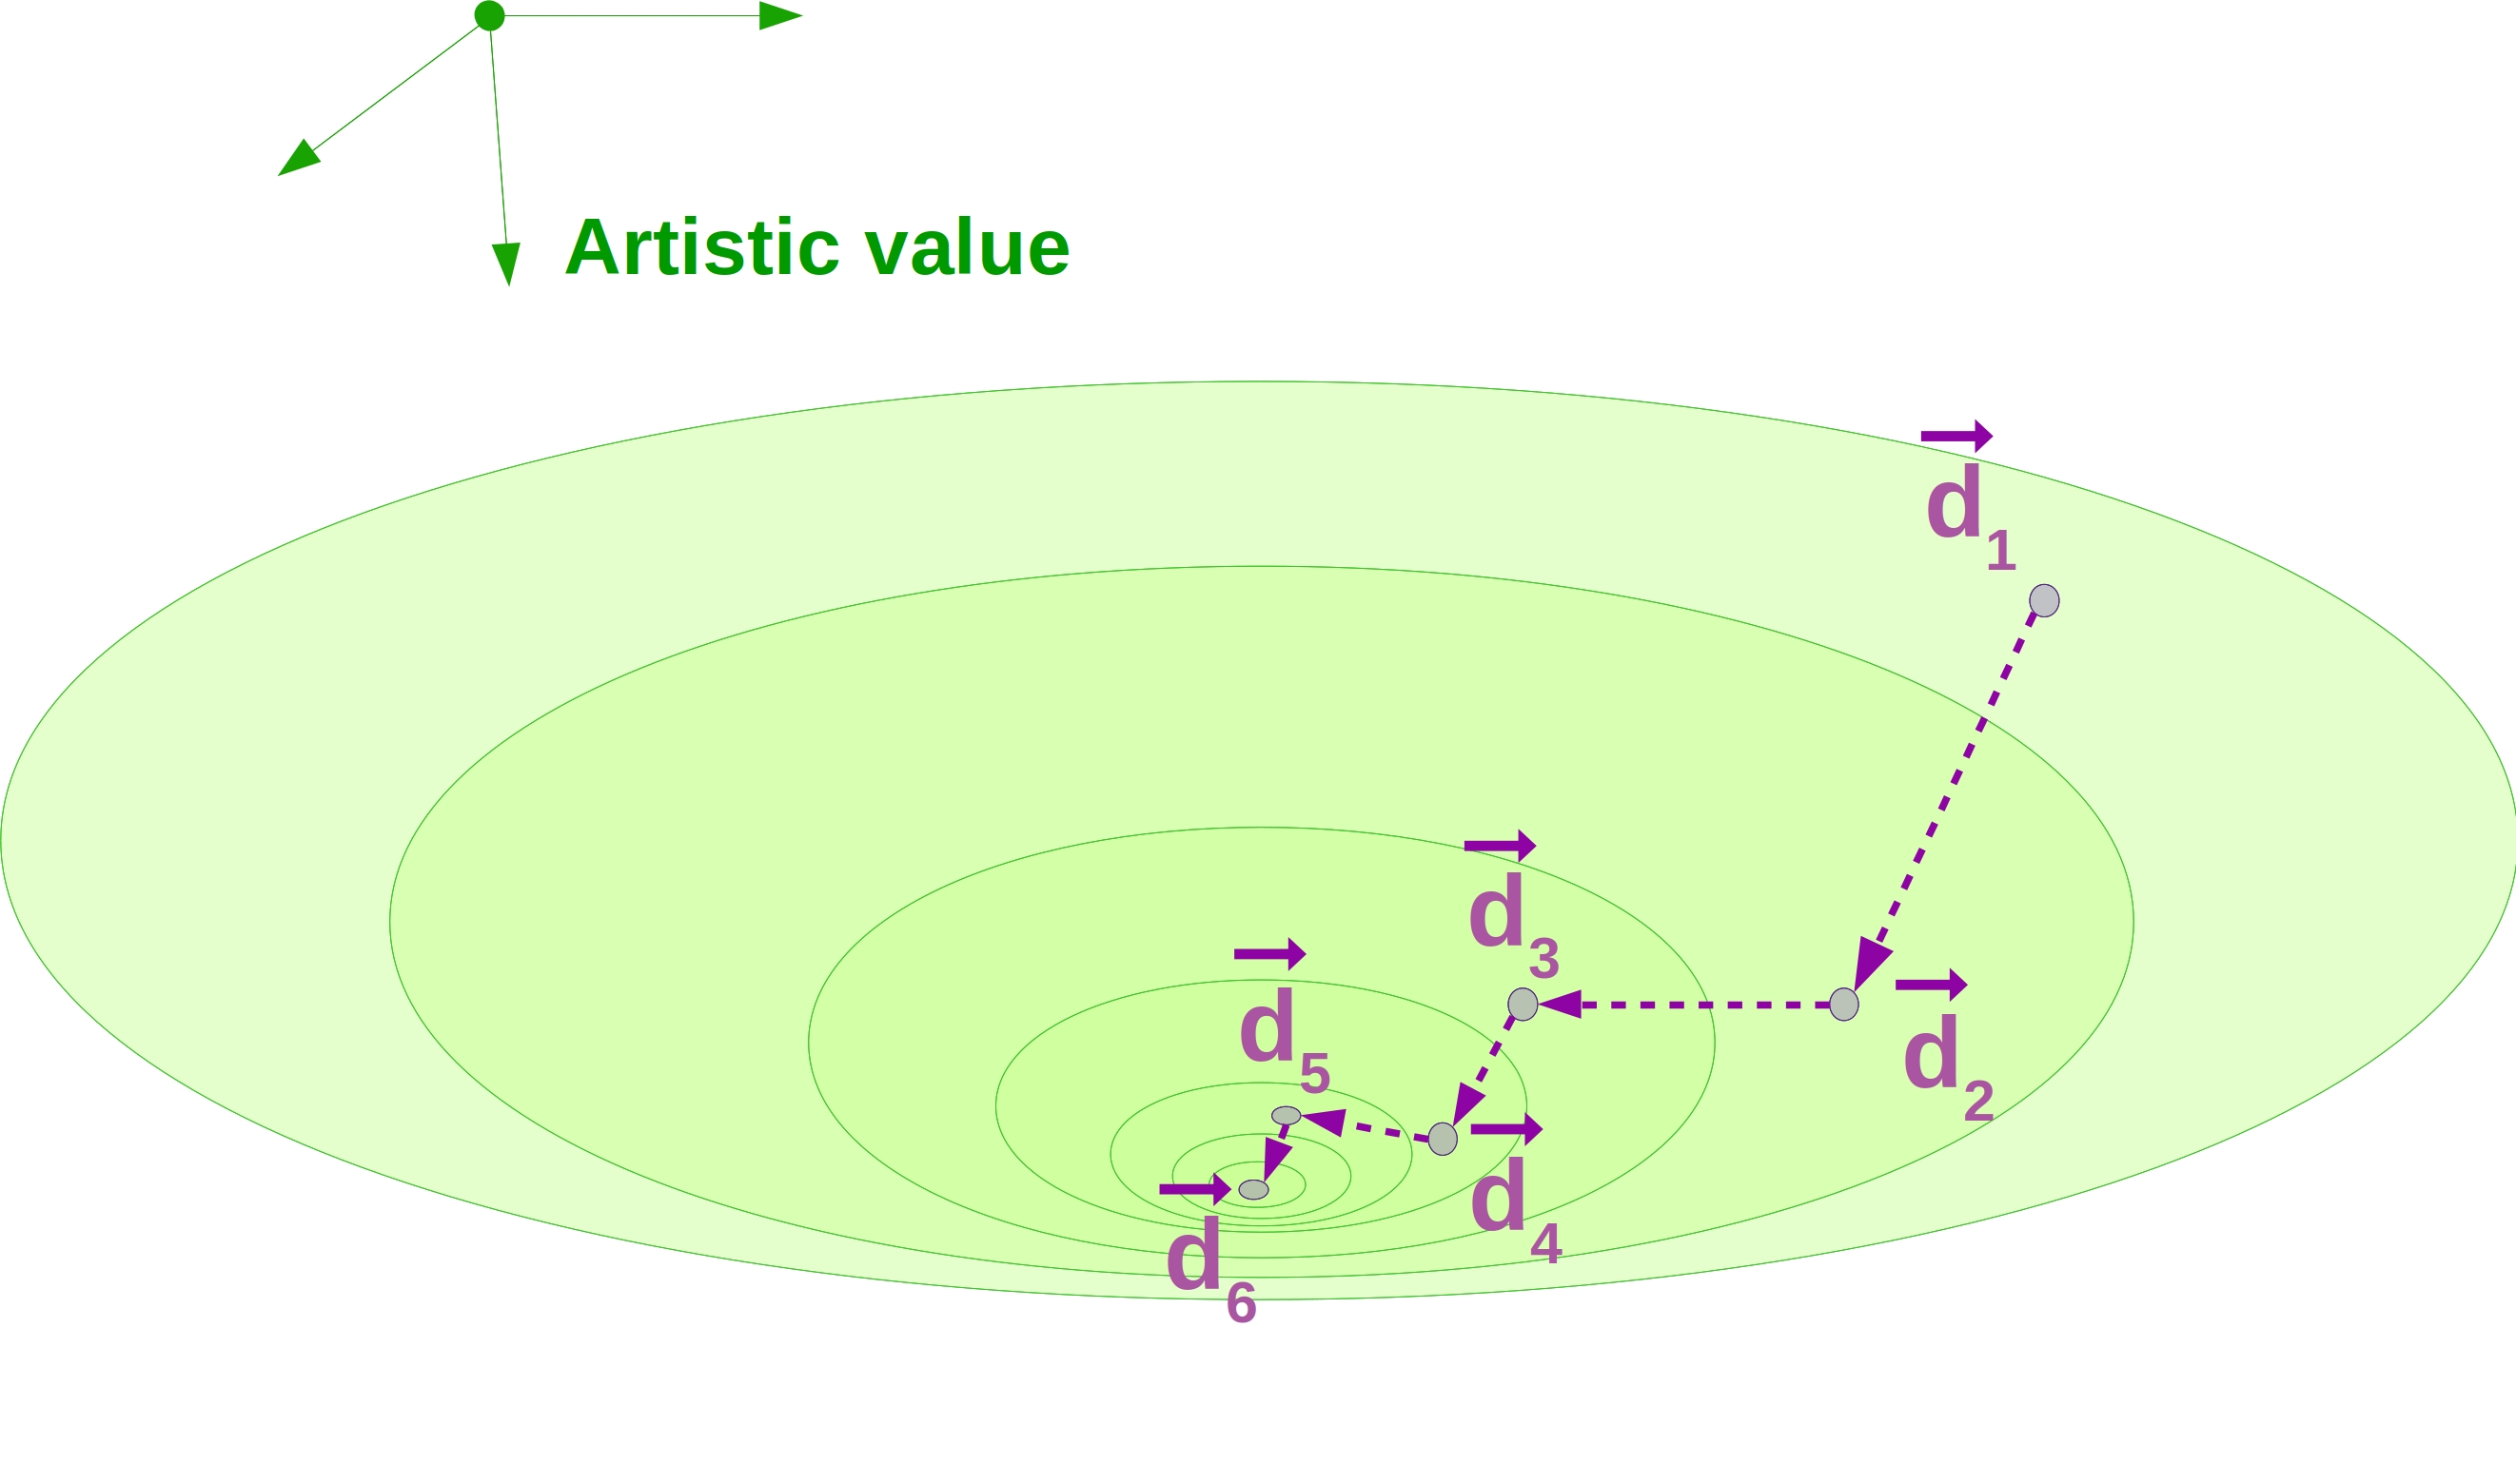
\includegraphics[width=0.6\textwidth]{/media/donkarlo/Elements/projs/research/assets/dependency-sequence-gradient-descent.jpg}
		\caption{Dependencies from $\vec{d_1}$ to $\vec{d_6}$ where the maximum artistic value of all indexes in Section \ref{sec:methodology-artistic value-indexes} happen. If $\vec{d_1}$ was happen to be chosen in another location or the stochastic gradient descent on Equation \ref{eq:comprehensive-artistic-function} repeats, certainly another sequence of dependencies with a different length would be introduced.} 
		\label{fig:dependency-gradient-descent}
	\end{figure}	
	\subsection{Surface realization from dependencies}
	In this phase, the dependency sequences generated in Section \ref{sec:methodology-stochastic-gradient-descent} will be converted to real natural language sentences by either taking advantage of methods introduced in Section \ref{sec:related-works-surface-realization} or more approaches tailored to the particular requirements of this proposal. 
	
	\section{Baselines and evaluation} \label{sec:baselines-evaluations}
	\subsection{Baseline}
	\citet{mcintyre-2009-learning-to-tell-tales-a-data-driven-approach-to-story-generation, mcintyre-2010-plot-induction-and-evolutionary-search-for-story-generation} introduce psycho-linguistic methods as an index for interestingness. Their solution fits as a baseline model for this proposal because it also functions based on joining dependencies derived from corpora by either a rank or evolutionary based models to choose the appropriate dependent sequence among a set of dependency population such as $D$. 
	\subsection{Artistic value index detector models} \label{sec:baselines-evaluations-artistic value-indexes}
	If the model in Section  \ref{sec:methodology-stochastic-gradient-descent} generates n dependency sequences then:
	\paragraph{Antonym class shifts detector model:} If the antonym detector in the model in Section \ref{sec:methodology-antonym-class-shifts} detects $t$ haiku with antonyms, (considering the fact that all haiku include antonym semantic class shift) then we expect 
	\begin{equation}
	n \times \frac{|A|}{t}
	\end{equation}
	of dependency sequences generated by the method in Section \ref{sec:methodology-stochastic-gradient-descent} must include at least one antonym shift other wise the model must be improved. 
	\paragraph{Ambiguity and VAD gravity} The same rules or antonym detector model, applies to ambiguity and VAD gravity models, although finding corpora for these two indexes is more challenging.  
	\subsection{Human evaluation} 
	This is one of the rare cases in natural language generation where machine evaluation techniques which were described in Section \ref{sec:baselines-evaluations-artistic value-indexes} may work better since artistic value qualities are hard to judge by human agents according to their understanding of art but the proposed approach is based on mathematical definition of artistic indexes which are more strict. Overall, human evaluation will be used to find out how close machine and human judgments are in this area. 
	\subsection{Surface realization} 
	Using methods such as BLEU \citep{papineni-2002-bleu-a-method-for-automatic-evaluation-of-machine-translation} or METEOR \citep{lavie-2007-proceedings-of-the-acl-workshop-on-intrinsic-and-extrinsic-evaluation-measures-for-machine-translation-and-or-summarization} the final results in natural language could be evaluated. Yet, human evaluation on final results is also an asset for overall assessment of the model's performance. %todo are there any poem evaluator?%
	
	\section{Timetable}
	\begin{itemize}
		\item Phase 1: 4 months: Choosing the corpora and dependency extraction from an unbiased corpus	
		\item Phase 2: 9 months: Developing models to cluster words antonym words into different semantic classes and detect semantic antonym shifts in a sequence of dependencies
		\item Phase 3: 10 months: Developing models that can cluster words according to their meaning and detect ambiguity appeal of a sequence of dependencies
		\item Phase 5: 10 months: Developing a model that can detect historical VAD of the final semantic class in which a sequence of dependencies has resided. 
		\item Phase 6: 9 months: Stochastic Gradient descent implementation to generate dependency sequences with maximum artistic indexes described in three previous phases. 
		\item Phase 7: 6 months: making improvements iterations in previous stages and trying to add supplementary artistic indexes. 
	\end{itemize}
	\section{Papers}
	During the PhD these papers should be published to accomplish the objective and the road map sketched in methodology section. 
	\begin{itemize} 
		\item A paper will be developed to present the results of clustering antonym words into different classes and detecting semantic antonym shifts at the end of phase two. Probably a collection of haiku will be used to determine the performance of the antonym shifts detector model and present the results. 
		\item A paper will be developed to present the results of clustering the word embedding according to their meanings and detecting the ambiguity appeal of dependency sequences. 
		\item A paper will be developed to present the result of the VAD semantic vector space. 
		\item A paper with reference to three previous papers will be developed to present the results of dependency sequences introduced by stochastic gradient descent, introduced in Section \ref{sec:methodology-stochastic-gradient-descent} and evaluated according to the metrics described in Section \ref{sec:baselines-evaluations}.
	\end{itemize}
	\bibliography{/media/donkarlo/Elements/projs/research/refs}
\end{document}